% !TeX spellcheck = en_GB
%%%%%%%%%%%%%%%%%%%%%%%%%%%%%%%%%%%%%%%%%%
%                                        %
%    Engineer thesis LaTeX template      %
%  compliant with the SZJK regulations   %
%                                        %
%%%%%%%%%%%%%%%%%%%%%%%%%%%%%%%%%%%%%%%%%%
%                                        %
%  (c) Krzysztof Simiński, 2018-2022     %
%                                        %
%%%%%%%%%%%%%%%%%%%%%%%%%%%%%%%%%%%%%%%%%%
%                                        %
% The latest version of the templates is %
% available at                           %
% github.com/ksiminski/polsl-aei-theses  %
%                                        %
%%%%%%%%%%%%%%%%%%%%%%%%%%%%%%%%%%%%%%%%%%
%
%
% This LaTeX project formats the final thesis
% with compliance to the SZJK regulations.
% Please to not change formatting (fonts, margins,
% bolds, italics, etc).
%
% You can compile the project in several ways.
%
% 1. pdfLaTeX compilation
%
% pdflatex main
% bibtex   main
% pdflatex main
% pdflatex main
%
%
% 2. XeLaTeX compilation
%
% Compilation with the XeLaTeX engine inserts Calibri font
% in the title page. Of course the font has to be installed.
%

% xelatex main
% bibtex  main
% xelatex main
% xelatex main
%
%
%%%%%%%%%%%%%%%%%%%%%%%%%%%%%%%%%%%%%%%%%%%%%%%%%%%%%%%%%%%%%%
% If you have any questions, remarks, just send me an email: %
%            krzysztof.siminski(at)polsl.pl               %
%%%%%%%%%%%%%%%%%%%%%%%%%%%%%%%%%%%%%%%%%%%%%%%%%%%%%%%%%%%%%%

% We would like to improve the LaTeX templates
% of final theses. By answering the questions
% in the survey whose address your can find below
% you help us to do so. The survey is completely
% anonimous. Thank you!
%
% https://docs.google.com/forms/d/e/1FAIpQLScyllVxNKzKFHfILDfdbwC-jvT8YL0RSTFs-s27UGw9CKn-fQ/viewform?usp=sf_link
%
%%%%%%%%%%%%%%%%%%%%%%%%%%%%%%%%%%%%%%%%%%%%%%%%%%%%%%%%%%%%%%%%%%%%%%%%%

%%%%%%%%%%%%%%%%%%%%%%%%%%%%%%%%%%%%%%%%%%%%%%%
%                                             %
% CUSTOMISATION OF THE THESIS                 %
%                                             %
%%%%%%%%%%%%%%%%%%%%%%%%%%%%%%%%%%%%%%%%%%%%%%%

% Please customise your thesis with the macros below.

% TODO
\newcommand{\Firstnames}{Daniel Bartosz}
\newcommand{\Surname}{Marek}
\newcommand{\Supervisor}{Jakub Nalepa PhD. DSc.}  % supervisor (remove $\langle$ and $\rangle)
\newcommand{\Title}{Extraterrestrial rock segmentation using machine learning}
\newcommand{\TitleAlt}{Segmentacja skał pozaziemskich z wykorzystaniem uczenia maszynowego}
\newcommand{\Program}{Informatics}
\newcommand{\Specialisation}{Computer Graphics and Software}
\newcommand{\Id}{290763} %  (remove $\langle$ and $\rangle)
\newcommand{\Departament}{Department of Algorithmics and Software } % your supervisor's departament  (remove $\langle$ and $\rangle)


% If you have a consultant for your thesis, put their name below ...
\newcommand{\Consultant}{title first name surname}  %  (remove $\langle$ and $\rangle)
% ... else leave the braces empty:
%\newcommand{\consultant}{} % no consultant

% end of thesis customisation
%%%%%%%%%%%%%%%%%%%%%%%%%%%%%%%%%%%%%%%%%%

%%%%%%%%%%%%%%%%%%%%%%%%%%%%%%%%%%%%%%%%%%%%%%%
%                                             %
% END OF CUSTOMISATION                        %
%                                             %
%%%%%%%%%%%%%%%%%%%%%%%%%%%%%%%%%%%%%%%%%%%%%%%

%%%%%%%%%%%%%%%%%%%%%%%%%%%%%%%%%%%%%%%%


%%%%%%%%%%%%%%%%%%%%%%%%%%%%%%%%%%%%%%%%%%%%%%%
%                                             %
%   PLEASE DO NOT MODIFY THE SETTINGS BELOW!  %
%                                             %
%%%%%%%%%%%%%%%%%%%%%%%%%%%%%%%%%%%%%%%%%%%%%%%



\documentclass[a4paper,twoside,12pt]{book}
\usepackage[utf8]{inputenc}
\usepackage[T1]{fontenc}
\usepackage{amsmath,amsfonts,amssymb,amsthm}
\usepackage[polish,british]{babel}
\usepackage{indentfirst}



\usepackage{ifxetex}

\ifxetex
	\usepackage{fontspec}
	\defaultfontfeatures{Mapping=tex—text} % to support TeX conventions like ``——-''
	\usepackage{xunicode} % Unicode support for LaTeX character names (accents, European chars, etc)
	\usepackage{xltxtra} % Extra customizations for XeLaTeX
\else
	\usepackage{lmodern}
\fi



\usepackage[margin=2.5cm]{geometry}
\usepackage{graphicx}
\usepackage{hyperref}
\usepackage{booktabs}
\usepackage{tikz}
\usepackage{pgfplots}
\usepackage{mathtools}
\usepackage{geometry}
\usepackage{subcaption}   % subfigures
\usepackage[page]{appendix} % toc,




\usepackage{csquotes}
\usepackage[natbib=true,backend=bibtex,maxbibnames=99]{biblatex}  % compilation of bibliography with BibTeX
%\usepackage[natbib=true,backend=biber,maxbibnames=99]{biblatex}  % compilation of bibliography with Biber
\bibliography{biblio}

\usepackage{ifmtarg}   % empty commands

\usepackage{setspace}
\onehalfspacing


\frenchspacing



%%%% TODO LIST GENERATOR %%%%%%%%%

\usepackage{color}
\definecolor{brickred}      {cmyk}{0   , 0.89, 0.94, 0.28}

\makeatletter \newcommand \kslistofremarks{\section*{Remarks} \@starttoc{rks}}
  \newcommand\l@uwagas[2]
    {\par\noindent \textbf{#2:} %\parbox{10cm}
{#1}\par} \makeatother


\newcommand{\ksremark}[1]{%
{%\marginpar{\textdbend}
{\color{brickred}{[#1]}}}%
\addcontentsline{rks}{uwagas}{\protect{#1}}%
}










%%%%%%%%%%%%%% END OF TODO LIST GENERATOR %%%%%%%%%%%

%%%%%%%%%%%% FANCY HEADERS %%%%%%%%%%%%%%%
% no capitalisation of headers
\usepackage{fancyhdr}
\pagestyle{fancy}
\fancyhf{}
\fancyhead[LO]{\nouppercase{\it\rightmark}}
\fancyhead[RE]{\nouppercase{\it\leftmark}}
\fancyhead[LE,RO]{\it\thepage}


\fancypagestyle{onlyPageNumbers}{%
   \fancyhf{}
   \fancyhead[LE,RO]{\it\thepage}
}

\fancypagestyle{noNumbers}{%
   \fancyhf{}
   \fancyhead[LE,RO]{}
}


\fancypagestyle{PageNumbersChapterTitles}{%
   \fancyhf{}
   \fancyhead[LO]{\nouppercase{\Firstnames\ \Surname}}
   \fancyhead[RE]{\nouppercase{\leftmark}}
   \fancyfoot[CE, CO]{\thepage}
}




%%%%%%%%%%%%%%%%%%%%%%%%%%%







\newcounter{pagesWithoutNumbers}

%%%%%%%%%%%%%%%%%%%%%%%%%%%
\usepackage{xstring}
\usepackage{ifthen}
\newcommand{\printOpiekun}[1]{%

    \StrLen{\Consultant}[\mystringlen]
    \ifthenelse{\mystringlen > 0}%
    {%
       {\large{\bfseries CONSULTANT}\par}

       {\large{\bfseries \Consultant}\par}
    }%
    {}
}
%
%%%%%%%%%%%%%%%%%%%%%%%%%%%%%%%%%%%%%%%%%%%%%%

% Please do not modify the lines below!
\author{\Firstnames\ \Surname}
\newcommand{\Author}{\Firstnames\ \MakeUppercase{\Surname}}
\newcommand{\Type}{FINAL PROJECT}
\newcommand{\Faculty}{Faculty of Automatic Control, Electronics and Computer Science}
\newcommand{\Polsl}{Silesian University of Technology}
\newcommand{\Logo}{politechnika_sl_logo_bw_pion_en.pdf}
\newcommand{\LeftId}{Student identification number}
\newcommand{\LeftProgram}{Programme}
\newcommand{\LeftSpecialisation}{Specialisation}
\newcommand{\LeftSUPERVISOR}{SUPERVISOR}
\newcommand{\LeftDEPARTMENT}{DEPARTMENT}
%%%%%%%%%%%%%%%%%%%%%%%%%%%%%%%%%%%%%%%%%%%%%%

%%%%%%%%%%%%%%%%%%%%%%%%%%%%%%%%%%%%%%%%%%%%%%%
%                                             %
% END OF SETTINGS                             %
%                                             %
%%%%%%%%%%%%%%%%%%%%%%%%%%%%%%%%%%%%%%%%%%%%%%%




%%%%%%%%%%%%%%%%%%%%%%%%%%%%%%%%%%%%%%%%%%%%%%%
%                                             %
% MY PACKAGES, SETTINGS ETC.                  %
%                                             %
%%%%%%%%%%%%%%%%%%%%%%%%%%%%%%%%%%%%%%%%%%%%%%%

% Put your packages, macros, setting here.



%%%%%%%%%%%%%%%%%%%%%%%%%%%%%%%%%%%%%%%%%%%%%%%%%%%%%%%%%%%%%%%%%%%%%
% listings
% packages: listings or minted
% % % % % % % % % % % % % % % % % % % % % % % % % % % % % % % % % % %

% package listings
\usepackage{listings}
\lstset{%
morekeywords={string,exception,std,vector},% add the keyword you need
language=C++,% C, Matlab, Python, SQL, TeX, XML, bash, ... – vide https://www.ctan.org/pkg/listings
commentstyle=\textit,%
identifierstyle=\textsf,%
keywordstyle=\sffamily\bfseries, %\texttt, %
%captionpos=b,%
tabsize=3,%
frame=lines,%
numbers=left,%
numberstyle=\tiny,%
numbersep=5pt,%
breaklines=true,%
%morekeywords={descriptor_gaussian,descriptor,partition,fcm_possibilistic,dataset,my_exception,exception,std,vector},%
escapeinside={@*}{*@},%
}

% % % % % % % % % % % % % % % % % % % % % % % % % % % % % % % % % % %
% package minted
% \usepackage{minted}

% This package requires a special command line option in compilation
% pdflatex -shell-escape main.tex
% xelatex  -shell-escape main.tex

%%%%%%%%%%%%%%%%%%%%%%%%%%%%%%%%%%%%%%%%%%%%%%%%%%%%%%%%%%%%%%%%%%%%%



%%%%%%%%%%%%%%%%%%%%%%%%%%%%%%%%%%%%%%%%%%%%%%%
%                                             %
% END OF MY PACKAGES, SETTINGS ETC.           %
%                                             %
%%%%%%%%%%%%%%%%%%%%%%%%%%%%%%%%%%%%%%%%%%%%%%%



%%%%%%%%%%%%%%%%%%%%%%%%%%%%%%%%%%%%%%%%


\begin{document}
%\kslistofremarks


%%%%%%%%%%%%%%%%%%%%%%%%%%%%%%%%%%%%%%%%%%%%%%%
%                                             %
%    PLEASE DO NOT MODIFY THE TITLE PAGE!     %
%                                             %
%%%%%%%%%%%%%%%%%%%%%%%%%%%%%%%%%%%%%%%%%%%%%%%


%%%%%%%%%%%%%%%%%%  TITLE PAGE %%%%%%%%%%%%%%%%%%%
\pagestyle{empty}
{
	\newgeometry{top=1.5cm,%
	             bottom=2.5cm,%
	             left=3cm,
	             right=2.5cm}

	\ifxetex
	  \begingroup
	  \setsansfont{Calibri}

	\fi
	 \sffamily
	\begin{center}
	\includegraphics[width=50mm]{\Logo}


	{\Large\bfseries\Type\par}

	\vfill  \vfill

	{\large\Title\par}

	\vfill

	{\large\bfseries\Author\par}

	{\normalsize\bfseries \LeftId: \Id}

	\vfill

	{\large{\bfseries \LeftProgram:} \Program\par}

	{\large{\bfseries \LeftSpecialisation:} \Specialisation\par}

	\vfill  \vfill 	\vfill 	\vfill 	\vfill 	\vfill 	\vfill

	{\large{\bfseries \LeftSUPERVISOR}\par}

	{\large{\bfseries \Supervisor}\par}

	{\large{\bfseries \LeftDEPARTMENT\ \Departament}\par}

	{\large{\bfseries \Faculty}\par}

	\vfill  \vfill


    \printOpiekun{\Consultant}

	\vfill  \vfill

    {\large\bfseries  Gliwice \the\year}

   \end{center}
       \ifxetex
       	  \endgroup
       \fi
	\restoregeometry
}



\cleardoublepage

\rmfamily\normalfont
\pagestyle{empty}


%%% Let's start the thesis %%%%

% TODO
\subsubsection*{Thesis title}
\Title

\subsubsection*{Abstract}
(Thesis abstract – to be copied into an appropriate field during an electronic submission – in English.)

\subsubsection*{Key words}
(2-5 keywords, separated by commas)

\subsubsection*{Tytuł pracy}
\begin{otherlanguage}{polish}
\TitleAlt
\end{otherlanguage}

\subsubsection*{Streszczenie}
\begin{otherlanguage}{polish}
(Streszczenie pracy – odpowiednie pole w systemie APD powinno zawierać kopię tego streszczenia.)
\end{otherlanguage}

\subsubsection*{Słowa kluczowe}
\begin{otherlanguage}{polish}
(2-5 slow (fraz) kluczowych, oddzielonych przecinkami)
\end{otherlanguage}




%%%%%%%%%%%%%%%%%% Table of contents %%%%%%%%%%%%%%%%%%%%%%
%\pagenumbering{Roman}
\thispagestyle{empty}
\tableofcontents
\thispagestyle{empty}

%%%%%%%%%%%%%%%%%%%%%%%%%%%%%%%%%%%%%%%%%%%%%%%%%%%%%
\setcounter{pagesWithoutNumbers}{\value{page}}
\mainmatter
\pagestyle{empty}

\cleardoublepage

\pagestyle{PageNumbersChapterTitles}

%%%%%%%%%%%%%% body of the thesis %%%%%%%%%%%%%%%%%

% TODO
\chapter{Introduction}
In 1969 during the Apollo 11 mission, humanity reached the Moon for the first time in history. This phenomenal achievement was possible thanks to countless hours of hard work put in by the brightest engineers and scientists of that time. It was proven possible to reach a new world. The last time humans stood on the Moon was during the Apollo 17 mission in 1972. Since the end of the space race, many uncrewed missions have studied the core and surface of the silver globe. In 2017 a new Moon exploration program led by the United States National Aeronautics and Space Administration was launched. This program aims to reestablish a human presence on the Moon, with the long-term goal of creating a permanent base camp and facilitating human missions to Mars.

Establishing a human presence on another world is challenging due to cosmic radiation, lack of breathable air, high temperature fluctuations and many environmental hazards. Specialized space exploration vehicles, such as lunar or planetary rovers, are created to work in such harsh conditions. Rovers perform various tasks, including collecting information about the terrain they landed on, collecting soil or rock samples, testing equipment for future missions, or simply sending back photos of their surroundings.  Since rovers are meant to land on celestial bodies far from earth, it is impossible to remotely control them in real time due to the speed of radio signal transmission. Therefore, such machines require full or partial autonomy to operate efficiently. Currently, rovers are only partially autonomous, relying on the ground control team for operation. Achieving significant or full autonomy would result in greater efficiency and performance in completing tasks regarding space exploration.

Autonomous tasks performed by exploration rovers could include navigation around terrain, including path planning, hazard detection and objects of interest detection, as well as efficient power consumption, data transfer and positioning for recharging with solar energy. Extreme environmental conditions impose strict regulations on rover design to ensure extended and flawless workings, meaning that all electronic parts are adequately shielded and protected. Due to those limitations, computers controlling all functionality are restricted to microprocessors with limited performance. Software performing all rover functionality while maintaining low power consumption requires high optimisation levels and well-thought-out architecture. Additionally, equipping the robot with autonomy may be problematic for classical algorithms. To overcome these restrictions, machine learning-based algorithms can be employed.

% Tutaj nie jestem pewien co do tych dwóch akapitów, na ile rozpisywać się o tej historii i szczegółach.
In the 20th century, when computers were not as powerful as today, a debate arose on achieving intelligence using computers. The first approach was to use logic and symbolic representation so intelligent systems could reason about the word, known as Symbolic Artificial Intelligence. The second approach was to achieve intelligence through learning, known as the connectionist approach. Due to intellectual traditions and hardware limitations, Symbolic Artificial Intelligence won over the connectionist approach, forcing programmers to write long and complicated programs for every problem they encountered. Solutions based on the connectionist approach emerged again in the early 21st century in the form of deep learning based on neural networks, which were developed back in the 1980s by scientists from different fields inspired by biological brain learning capability. Increased computing resources and available data caused deep learning methods to dominate in accuracy benchmarks around 2012.

Since 2015, deep learning has been widely used in various ways, especially in computer vision, as correct classification or detection of objects in photos has begun to surpass an average human's accuracy. Solutions based on deep learning are mostly used in powerful data centres as sophisticated state-of-the-art algorithms are consuming a significant amount of computing resources. The fact that deep learning models are resource expensive to train but efficient with inference led to more extensive use with mobile technologies. A solution called "Edge AI" has been gaining popularity recently. It unlocks a whole new area of machine learning applications, enabling faster inference, lower energy consumption and not requiring connection to powerful servers. This approach can be applied to both computers with less powerful hardware, as well as to microcontrollers. There are numerous machine learning applications in embedded devices, such as smart assistants, self-driving cars, autonomous mobile robots and many more.
% Tutasj może trochę wrócić do poprzedniego tematu tak aby przejście było nieco bardziej płynne


\section{Motivation and goal of the project}
The development of fully autonomous lunar and planetary rovers will significantly enhance the speed of space exploration. Sensors and cameras that rovers are equipped with are sufficient for ground control to gain information about the rovers' surroundings. Recent advances in machine learning make it possible to process that information on board the vehicle, enabling autonomous navigation, hazard avoidance and decision-making, skipping the communication process with the control team. To comply with limited rover hardware and power draw, algorithms designed for onboard work must be as compact and efficient as possible. Inspection of the surroundings can be performed with semantic segmentation algorithms, which means assigning a class to every input image pixel. All known extraterrestrial surfaces worth exploring are mostly filled with rocks of different sizes, meaning detecting where rocks are located near the vehicle is crucial for autonomous navigation.

This work focuses on employing a machine learning algorithm based on state-of-the-art approaches to performing semantic segmentation on rocks in images of extraterrestrial landscapes. The main goal is to create an algorithm that is as accurate as possible while remaining compact and efficient. The trade-off between accuracy and compactness is crucial when designing an algorithm for embedded devices, especially considering the constraints of rover hardware design. The training is performed on an artificial lunar landscape data set using efficient hardware. Inference results of such an algorithm can be later used by other algorithms concerning tasks such as path planning, navigation or detecting objects of interest.

\section{Project overview}
This work is divided into three main parts: the first part is the theoretical introduction, the second part is the overview of the engineering part, the third part presents the obtained results, and the fourth part contains the conclusion.


The theoretical introduction is realised in the first chapter, where the domain is presented, as well as the motivation and how the problem is settled. Here, an outline of related works is presented. The engineering part is illustrated in the second chapter. An in-depth analysis of the methods used is performed, along with the presentation of how data is processed in order to obtain expected results. The results are presented in the third chapter. The chapter is laid out in the following manner: first, the preliminary results are presented, then the results after changing the architecture and what the motivation was, and the final results are presented at the end. The conclusions, general remarks and future work is presented in the final chapter.
%Tutaj jeszcze nie jestem pewnie co dokładnie opisać, wstępnie o tym że praca ma 3 części - teoretyczne wprowadzenie, wstępne wyniki oraz dokładniejsze wyniki

\section{Related works}
% @TODO: naprawić kolejność bibliografi
The importance of using artificial intelligence in space applications is presented in \cite{chien2006future}, as the authors focus on more future missions. How robotics and autonomous systems are currently used in space exploration is reviewed in \cite{gao2017review} and presents the history and future of robotic space missions, focusing on planetary missions. The authors concentrate on the importance of autonomy in these missions. The overview of what goals martian rovers have to achieve and how to use available sensors for autonomous operation is presented in \cite{bajracharya2008autonomy}. A survey of work applicable to autonomous planetary rover navigation is presented in \cite{wong2017adaptive}, where different ongoing challenges and promising future research directions are outlined.

Another work touching on rock segmentation is \cite{kuang2021rock}, where authors present a deep learning algorithm for use in the navigation vision of martian planetary rovers. In this article, the authors present their synthetic data set for segmentation, created using the Katwijk beach planetary rover data set \cite{hewitt2018katwijk}. Although the data used in this work is different, it is suitable as a reference point for comparing the results of obtained algorithms using similar metrics.

Classifying pixels of images obtained by rovers is also presented in \cite{ono2015risk}. In this work, the authors use the random forest machine learning algorithm to perform semantic segmentation of images. Their work focuses on developing the algorithm for path planning and hazard detection in planetary rovers. This project uses images taken by the Curiosity rover, labelled by human experts. The importance of detecting rock in rover vision is highlighted by this work.

An extensive overview of image segmentation using deep learning is performed in \cite{minaee2021image}, providing insight into different aspects of more than 100 segmentation methods, including the training data, loss functions, choice of architecture and key contributions. The review of the most significant state-of-the-art deep learning algorithms presented in this article serves as an entry port for choosing an optimal solution to the problem stated in this thesis. Another work providing deep insight into how to construct algorithms for image segmentation is \cite{ghosh2019understanding}. A paper focused on deep learning segmentation algorithms used in the more constrained environments is \cite{siam2018comparative}. An approach to designing computationally efficient solutions and a benchmarking framework for various algorithms are presented.

The edge computing deep learning algorithms are described in \cite{vestias2020moving}, along with the main research directions. This paper also presents several possible applications, including autonomous driving. A set of techniques used for optimising already existing algorithms in order to move them to the edge is laid down in this paper. A similar paper on how edge computing is \cite{merenda2020edge} focused more on running machine learning algorithms on microcontrollers.



% 1. ogólny zarys autonomi w misjach
% 2. segmentacji w łazikach
% 3. algorytmy segmentacji  ogólny zarys tutaj, konkretne enkodery oraz architektury potem
% 4. zastosowanie ai w embedded


% ====================================================
% \begin{itemize}
% \item introduction into the problem domain
% \item settling of the problem in the domain
% \item objective of the thesis
% \item scope of the thesis
% \item short description of chapters
% \item clear description of contribution of the thesis's author – in case of more authors table with enumeration of contribution of authors
% \end{itemize}
% ====================================================


\chapter{Task analysis}

\section{Data}
This work is mainly based on the Artificial Lunar Landscape data set, on which models are trained and assessed. Another data set containing label images for rocks on Mars have been introduced to further evaluate the generalisation ability of obtained algorithms.

\subsection{Artifical lunar landscape}
Artificial Lunar Dataset was created by Romain Pessia and Genya Ishigami of the Space Robotics Group, Keio University, Japan. This data set contains 9766 images of a photorealistic lunar environment made using the Terragen software. Images and ground truth segmentation masks are provided in files with matching names.

\begin{figure}[h!]
    \centering
    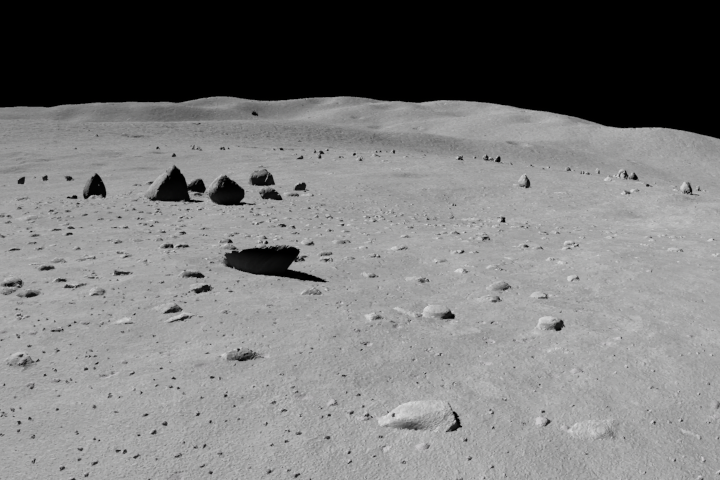
\includegraphics[width=5.5cm]{dataset_examples/Lunar/renders/render9679.png}
    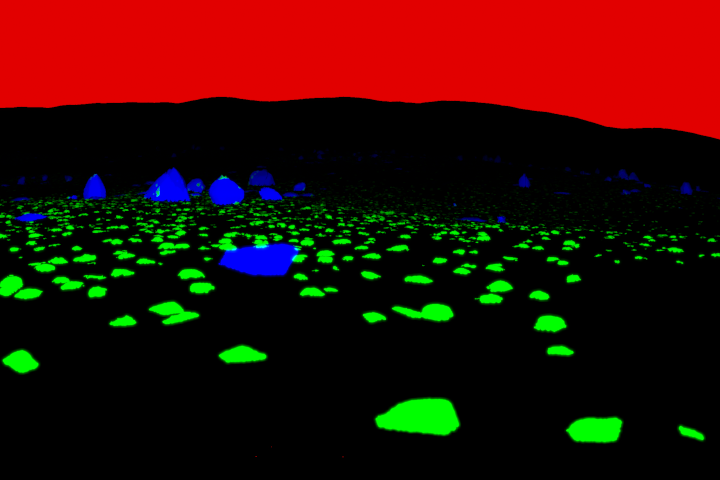
\includegraphics[width=5.5cm]{dataset_examples/Lunar/ground/ground9679.png}

    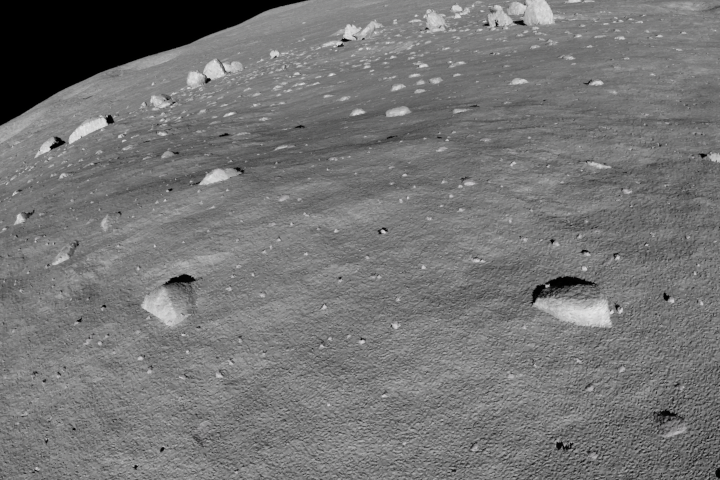
\includegraphics[width=5.5cm]{dataset_examples/Lunar/renders/render9723.png}
    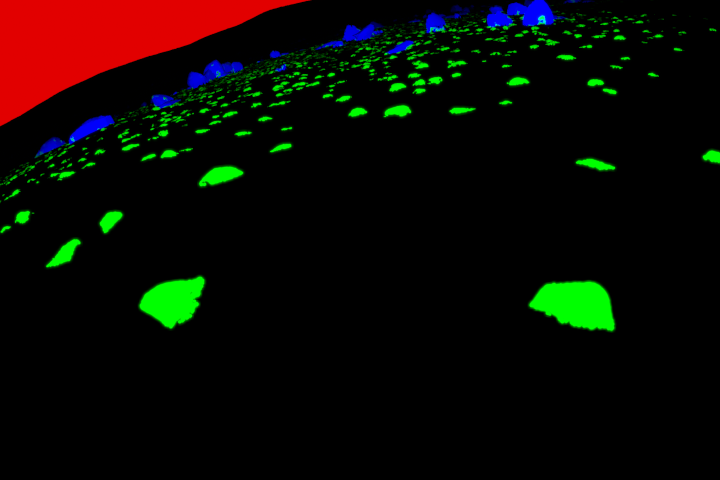
\includegraphics[width=5.5cm]{dataset_examples/Lunar/ground/ground9723.png}

    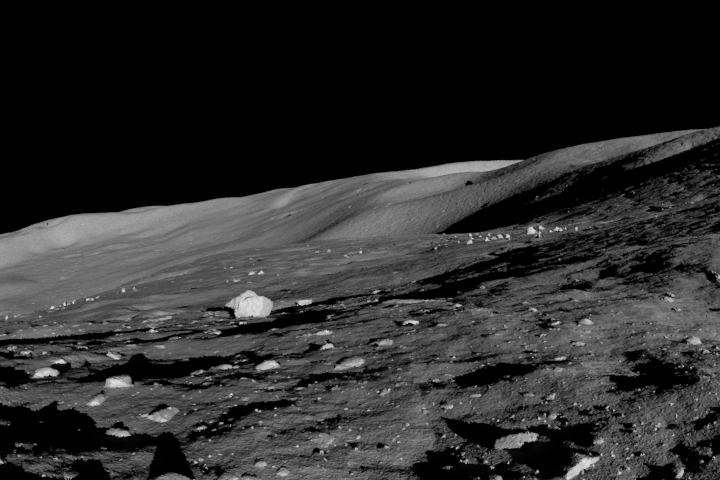
\includegraphics[width=5.5cm]{dataset_examples/Lunar/renders/render9688.png}
    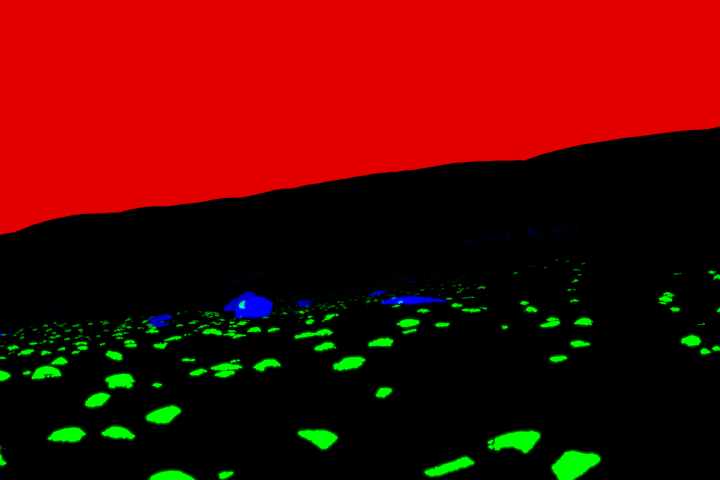
\includegraphics[width=5.5cm]{dataset_examples/Lunar/ground/ground9688.png}
    \caption{Example entries from data set with corresponding segmentation masks}
    \label{fig:data_example1}
\end{figure}

The resolution in which images are provided is $720 \times 480$ pixels. There are four segmentation classes available: large rocks (blue), smaller rocks (green), the sky (red) and everything else (black). The virtual camera capturing the renders is noise-free, and no data augmentation is performed. The position and rotation of the camera are random for each image, but the height with respect to the ground is kept low to mimic the rover's perspective. The heading and elevation of the sun are given random values for each image. Another significant property is that the colours of objects go darker with increased distance, meaning that setting the minimum intensity threshold for determining whether a certain rock should be considered is left to users. However, a threshold between 50 and 200 is recommended to avoid noise from distant rocks. Cleaned-up images of segmentation data where noise from smaller rocks is removed are also provided.

The authors also provide real lunar pictures taken by the Chang'e 3 rover equipped with two cameras to test algorithms trained on this data set. Hand-drew segmentation ground truth is also present for these pictures.

% TODO: naprawić pozycjonowanie tego szitu
\begin{figure}[!h]
    \centering
    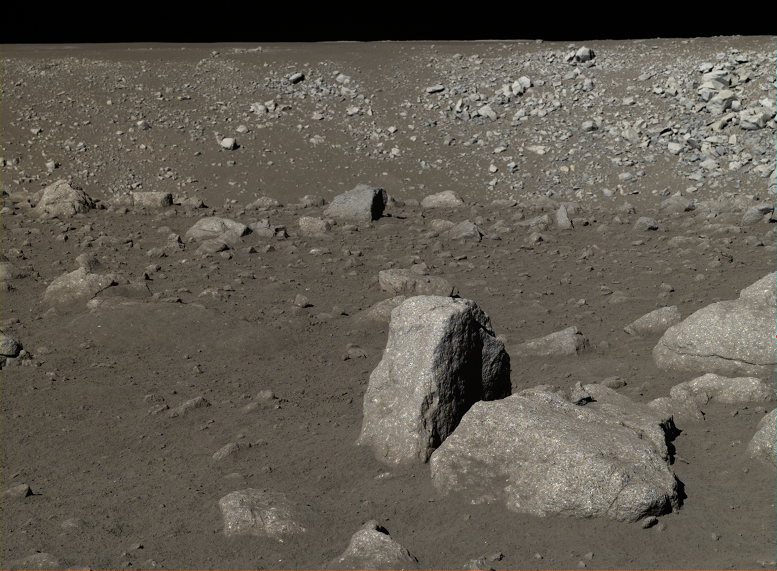
\includegraphics[width=5.5cm]{dataset_examples/Lunar/real/PCAM5.png}
    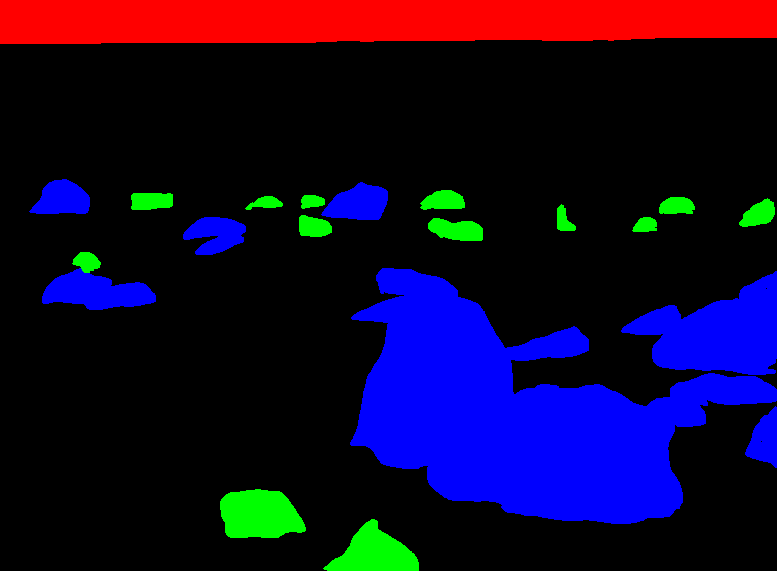
\includegraphics[width=5.5cm]{dataset_examples/Lunar/real/g_PCAM5.png}

    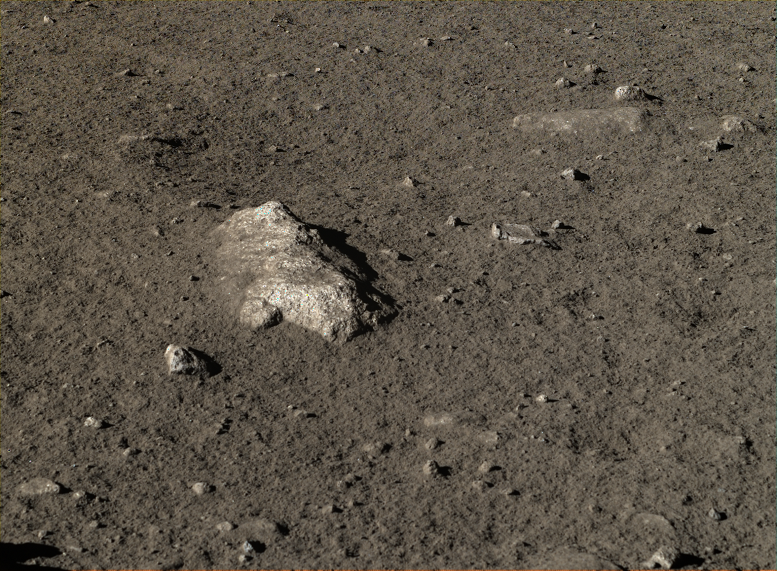
\includegraphics[width=5.5cm]{dataset_examples/Lunar/real/PCAM8.png}
    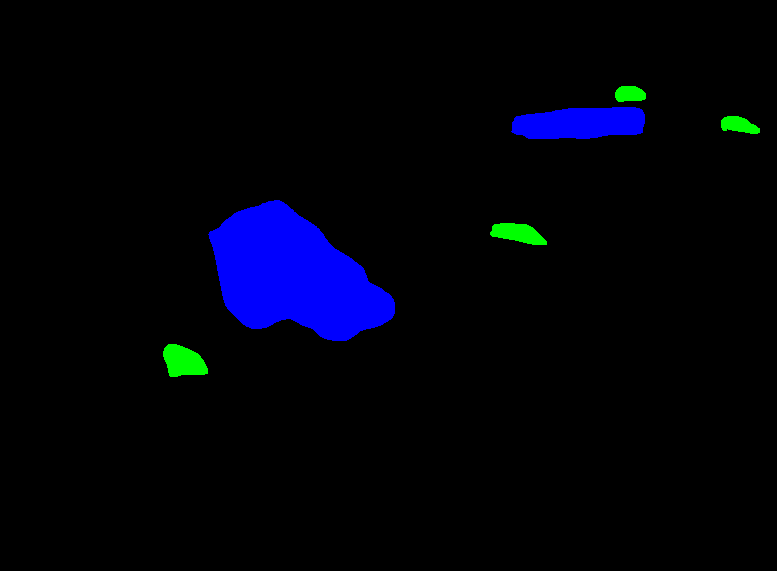
\includegraphics[width=5.5cm]{dataset_examples/Lunar/real/g_PCAM8.png}

    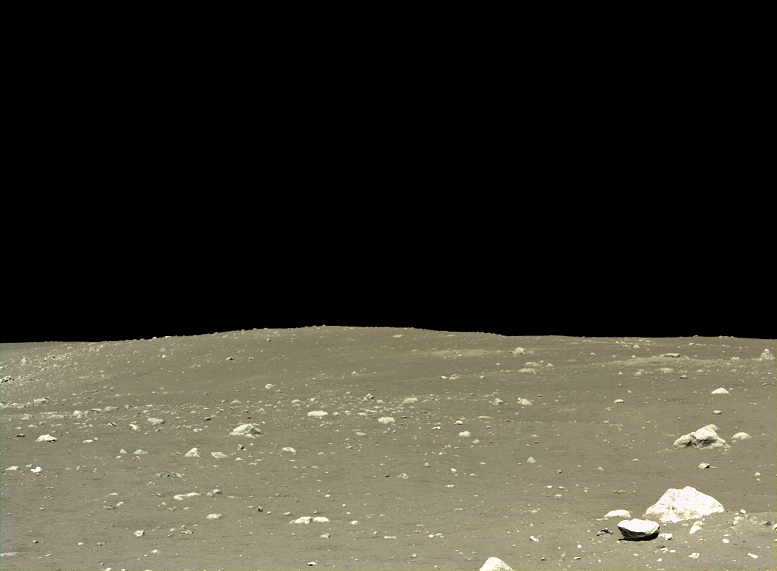
\includegraphics[width=5.5cm]{dataset_examples/Lunar/real/TCAM14.png}
    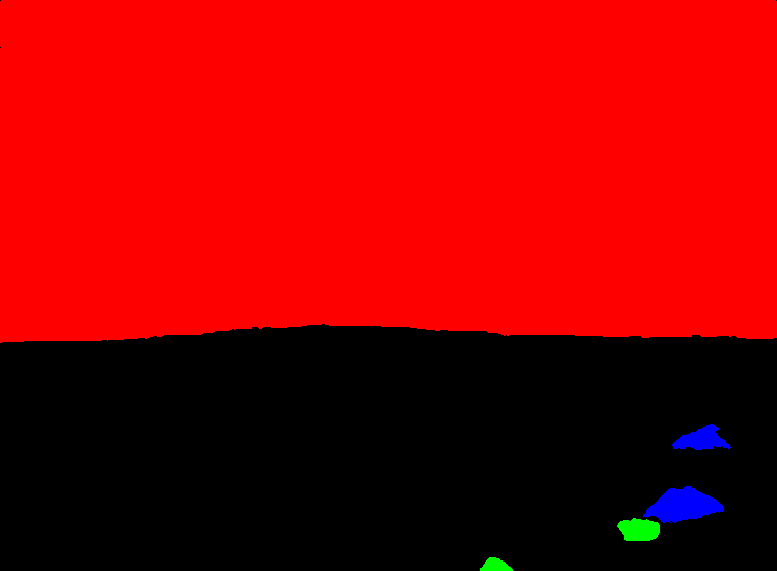
\includegraphics[width=5.5cm]{dataset_examples/Lunar/real/g_TCAM14.png}
    \caption{Example real lunar images with corresponding segmentation masks}
    \label{fig:data_real_example1}
\end{figure}

\subsection{Mars Data}
Mars Data \cite{xiao2021kernel} is a Martian rock segmentation dataset built using unlabeled images provided by NASA/JPL-Caltech. It is currently divided into two sub-datasets: Rock-A and Rock-B, with a total of 405 labelled rock images and more than 20000 rocks. Rock-A is a simpler sub-set, containing a few rocks in one image, while Rock-B is a more challenging sub-set with more abundant rocks in one scene. The authors also provide sets meant for model training and testing using data augmentation. All images are provided in $560 \times 500$ pixels resolution. Ground truth labels for this data set are only provided for binary segmentation, meaning that additional operations need to be performed in order to use this data.

\begin{figure}[!h]
    \centering
    \begin{subfigure}[b]{0.4\textwidth}
        \centering
        \includegraphics[width=3cm]{dataset_examples/Martian/Rock-A/image/964_0964ML0042700010403935E01_DXXX.jpg}
        \includegraphics[width=3cm]{dataset_examples/Martian/Rock-A/ground/964_0964ML0042700010403935E01_DXXX.png}

        \includegraphics[width=3cm]{dataset_examples/Martian/Rock-A/image/cr_116_0116MR0007330070200650E01_DXXX.jpg}
        \includegraphics[width=3cm]{dataset_examples/Martian/Rock-A/ground/cr_116_0116MR0007330070200650E01_DXXX.png}

        \includegraphics[width=3cm]{dataset_examples/Martian/Rock-A/image/cr_402_0402ML1667000000E1_DXXX.jpg}
        \includegraphics[width=3cm]{dataset_examples/Martian/Rock-A/ground/cr_402_0402ML1667000000E1_DXXX.png}

        \caption{Rock-A}
        \label{fig:rocka_martian_example}
    \end{subfigure}
    \begin{subfigure}[b]{0.4\textwidth}
        \centering
        \includegraphics[width=3cm]{dataset_examples/Martian/Rock-B/image/1580_1580ML0080490070604953E01_DXXX.jpg}
        \includegraphics[width=3cm]{dataset_examples/Martian/Rock-B/ground/1580_1580ML0080490070604953E01_DXXX.png}


        \includegraphics[width=3cm]{dataset_examples/Martian/Rock-B/image/cr_114_0114MR0006980120200632E01_DXXX.jpg}
        \includegraphics[width=3cm]{dataset_examples/Martian/Rock-B/ground/cr_114_0114MR0006980120200632E01_DXXX.png}

        \includegraphics[width=3cm]{dataset_examples/Martian/Rock-B/image/cr_714_0714MR0030410000402694E01_DXXX.jpg}
        \includegraphics[width=3cm]{dataset_examples/Martian/Rock-B/ground/cr_714_0714MR0030410000402694E01_DXXX.png}

        \caption{Rock-B}
        \label{fig:rockb_martian_example}
    \end{subfigure}
\caption{Examples martian images with corresponding segmentation masks}
\label{fig:martian_dataset_examples}
\end{figure}

\section{Tools}


% ====================================================
% \begin{itemize}
% \item  problem analysis
% \item state of the art, problem statement
% \item  literature research (all sources in the thesis have to be referenced \cite{bib:article,bib:book,bib:conference,bib:internet})
% \item description of existing solutions (also scientific ones, if the problem is scientifically researched), algorithms,  location of the thesis in the scientific domain
% \end{itemize}



% Mathematical formulae
% \begin{align}
% y = \frac{\partial x}{\partial t}
% \end{align}
% and single math symbols $x$ and $y$ are typeset in the mathematical mode.
% ====================================================


% TODO
\chapter{Requirements and tools}

\begin{itemize}
\item functional and nonfunctional requirements
\item use cases (UML diagrams)
\item description of tools
\item methodology of design and implementation
\end{itemize}

% TODO
\chapter{External specification}
\begin{itemize}
\item hardware and software requirements
\item installation procedure
\item activation procedure
\item types of users
\item user manual
\item system administration
\item security issues
\item example of usage
\item working scenarios (with screenshots or output files)
\end{itemize}




\begin{figure}
\centering
\begin{tikzpicture}
\begin{axis}[
    y tick label style={
        /pgf/number format/.cd,
            fixed,
            fixed zerofill, % 1.0 zamiast 1
            precision=1,
        /tikz/.cd
    },
    x tick label style={
        /pgf/number format/.cd,
            fixed,
            fixed zerofill,
            precision=2,
        /tikz/.cd
    }
]
\addplot [domain=0.0:0.1] {rnd};
\end{axis}
\end{tikzpicture}
\caption{Figure caption (below the figure).}
\label{fig:2}
\end{figure}

%%%%%%%%%%%%%%%%%%%%%
% FIGURE FROM FILE
%
%\begin{figure}
%\centering
%
\includegraphics[width=0.5\textwidth]{./politechnika_sl_logo_bw_pion_en.pdf}
%\caption{Caption of a figure is always below the figure.}
%\label{fig:label}
%\end{figure}
%Fig. \ref{fig:label} presents …
%%%%%%%%%%%%%%%%%%%%%
%
%%%%%%%%%%%%%%%%%%%%
%% SUBFIGURES
%
%\begin{figure}
%\centering
%\begin{subfigure}{0.4\textwidth}
%    
\includegraphics[width=\textwidth]{./politechnika_sl_logo_bw_pion_en.pdf}
%    \caption{Upper left figure.}
%    \label{fig:upper-left}
%\end{subfigure}
%\hfill
%\begin{subfigure}{0.4\textwidth}
%    
\includegraphics[width=\textwidth]{./politechnika_sl_logo_bw_pion_en.pdf}
%    \caption{Upper right figure.}
%    \label{fig:upper-right}
%\end{subfigure}
%
%\begin{subfigure}{0.4\textwidth}
%    
\includegraphics[width=\textwidth]{./politechnika_sl_logo_bw_pion_en.pdf}
%    \caption{Lower left figure.}
%    \label{fig:lower-left}
%\end{subfigure}
%\hfill
%\begin{subfigure}{0.4\textwidth}
%    
\includegraphics[width=\textwidth]{./politechnika_sl_logo_bw_pion_en.pdf}
%    \caption{Lower right figure.}
%    \label{fig:lower-right}
%\end{subfigure}
%
%\caption{Common caption for all subfigures.}
%\label{fig:subfigures}
%\end{figure}
%Fig. \ref{fig:subfigures} presents very important information, eg. Fig. \ref{fig:upper-right} is an upper right subfigure.
%%%%%%%%%%%%%%%%%%%%%


% TODO
\chapter{Internal specification}

\begin{itemize}
\item concept of the system
\item system architecture
\item description of data structures (and data bases)
\item components, modules, libraries, resume of important classes (if used)
\item resume of important algorithms (if used)
\item details of implementation of selected parts
\item applied design patterns
\item UML diagrams
\end{itemize}



% % % % % % % % % % % % % % % % % % % % % % % % % % % % % % % % % % %
% To use the minted packages uncomment the package import in        %
% file config/settings.tex :  \usepackage{minted}                   %
% and compile with the shell escape                                 %
% pdflatex -shell-escape main                                       %
% % % % % % % % % % % % % % % % % % % % % % % % % % % % % % % % % % %


Use special environments for inline code, eg  \lstinline|int a;| (package \texttt{listings})% or  \mintinline{C++}|int a;| (package \texttt{minted})
. Longer parts of code put in the figure environment, eg. code in Fig. \ref{fig:pseudocode:listings}% and Fig. \ref{fig:pseudocode:minted}
. Very long listings–move to an appendix.


\clearpage
\begin{figure}
\centering
\begin{lstlisting}
class test : public basic
{
    public:
      test (int a);
      friend std::ostream operator<<(std::ostream & s,
                                     const test & t);
    protected:
      int _a;

};
\end{lstlisting}
\caption{Pseudocode in \texttt{listings}.}
\label{fig:pseudocode:listings}
\end{figure}

%\begin{figure}
%\centering
%\begin{minted}[linenos,frame=lines]{c++}
%class test : public basic
%{
%    public:
%      test (int a);
%      friend std::ostream operator<<(std::ostream & s,
%                                     const test & t);
%    protected:
%      int _a;
%
%};
%\end{minted}
%\caption{Pseudocode in \texttt{minted}.}
%\label{fig:pseudocode:minted}
%\end{figure}




% TODO
\chapter{Verification and validation}
\begin{itemize}
\item testing paradigm (eg V model)
\item test cases, testing scope (full / partial)
\item detected and fixed bugs
\item results of experiments (optional)
\end{itemize}


\begin{table}
\centering
\caption{A caption of a table is \textbf{above} it.}
\label{id:tab:wyniki}
\begin{tabular}{rrrrrrrr}
\toprule
	         &                                     \multicolumn{7}{c}{method}                                      \\
	         \cmidrule{2-8}
	         &         &         &        \multicolumn{3}{c}{alg. 3}        & \multicolumn{2}{c}{alg. 4, $\gamma = 2$} \\
	         \cmidrule(r){4-6}\cmidrule(r){7-8}
	$\zeta$ &     alg. 1 &   alg. 2 & $\alpha= 1.5$ & $\alpha= 2$ & $\alpha= 3$ &   $\beta = 0.1$  &   $\beta = -0.1$ \\
\midrule
	       0 &  8.3250 & 1.45305 &       7.5791 &    14.8517 &    20.0028 & 1.16396 &                       1.1365 \\
	       5 &  0.6111 & 2.27126 &       6.9952 &    13.8560 &    18.6064 & 1.18659 &                       1.1630 \\
	      10 & 11.6126 & 2.69218 &       6.2520 &    12.5202 &    16.8278 & 1.23180 &                       1.2045 \\
	      15 &  0.5665 & 2.95046 &       5.7753 &    11.4588 &    15.4837 & 1.25131 &                       1.2614 \\
	      20 & 15.8728 & 3.07225 &       5.3071 &    10.3935 &    13.8738 & 1.25307 &                       1.2217 \\
	      25 &  0.9791 & 3.19034 &       5.4575 &     9.9533 &    13.0721 & 1.27104 &                       1.2640 \\
	      30 &  2.0228 & 3.27474 &       5.7461 &     9.7164 &    12.2637 & 1.33404 &                       1.3209 \\
	      35 & 13.4210 & 3.36086 &       6.6735 &    10.0442 &    12.0270 & 1.35385 &                       1.3059 \\
	      40 & 13.2226 & 3.36420 &       7.7248 &    10.4495 &    12.0379 & 1.34919 &                       1.2768 \\
	      45 & 12.8445 & 3.47436 &       8.5539 &    10.8552 &    12.2773 & 1.42303 &                       1.4362 \\
	      50 & 12.9245 & 3.58228 &       9.2702 &    11.2183 &    12.3990 & 1.40922 &                       1.3724 \\
\bottomrule
\end{tabular}
\end{table}



% TODO
\chapter{Conclusions}
\begin{itemize}
\item achieved results with regard to objectives of the thesis and requirements
\item path of further development (eg functional extension …)
\item encountered difficulties and problems
\end{itemize}



\backmatter

%\bibliographystyle{plain}  % bibtex
%\bibliography{biblio} % bibtex
\printbibliography           % biblatex
\addcontentsline{toc}{chapter}{References}

\begin{appendices}

% TODO

\chapter{Index of abbreviations and symbols}

\begin{itemize}
\item[DNA] deoxyribonucleic acid
\item[MVC] model--view--controller
\item[$N$] cardinality of data set
\item[$\mu$] membership function of a fuzzy set
\item[$\mathbb{E}$] set of edges of a graph
\item[$\mathcal{L}$] Laplace transformation
\end{itemize}


% TODO
\chapter{Listings}

(Put long listings here.)

\begin{lstlisting}
if (_nClusters < 1)
	throw std::string ("unknown number of clusters");
if (_nIterations < 1 and _epsilon < 0)
	throw std::string ("You should set a maximal number of iteration or minimal difference -- epsilon.");
if (_nIterations > 0 and _epsilon > 0)
	throw std::string ("Both number of iterations and minimal epsilon set -- you should set either number of iterations or minimal epsilon.");
\end{lstlisting}


% % % % % % % % % % % % % % % % % % % % % % % % % % % % % % % % % % %
% To use the minted packages uncomment the package import in        %
% file config/settings.tex :  \usepackage{minted}                   %
% and compile with the shell escape                                 %
% pdflatex -shell-escape main                                       %
% % % % % % % % % % % % % % % % % % % % % % % % % % % % % % % % % % %

%\begin{minted}[linenos,breaklines,frame=lines]{c++}
%if (_nClusters < 1)
%	throw std::string ("unknown number of clusters");
%if (_nIterations < 1 and _epsilon < 0)
%	throw std::string ("You should set a maximal number of iteration or minimal difference -- epsilon.");
%if (_nIterations > 0 and _epsilon > 0)
%	throw std::string ("Both number of iterations and minimal epsilon set -- you should set either number of iterations or minimal epsilon.");
%\end{minted}

% TODO
\chapter{List of additional files in~electronic submission (if applicable)}


Additional files uploaded to the system include:
\begin{itemize}
\item source code of the application,
\item test data,
\item a video file showing how software or hardware developed for thesis is used,
\item etc.
\end{itemize}

\listoffigures
\addcontentsline{toc}{chapter}{List of figures}
\listoftables
\addcontentsline{toc}{chapter}{List of tables}

\end{appendices}

\end{document}


%% Finis coronat opus.

